\documentclass[a4paper,11pt]{article}
\usepackage{amsmath,amsthm,amsfonts,amssymb,amscd,amstext,vmargin,graphics,graphicx,tabularx,multicol} 
\usepackage[francais]{babel}
\usepackage[utf8]{inputenc}  
\usepackage[T1]{fontenc} 
\usepackage{pstricks-add,tikz,tkz-tab,variations}
\usepackage[autolanguage,np]{numprint} 
\usepackage{calc}

\setmarginsrb{1.5cm}{0.5cm}{1cm}{0.5cm}{0cm}{0cm}{0cm}{0cm} %Gauche, haut, droite, haut
\newcounter{numexo}
\newcommand{\exo}[1]{\stepcounter{numexo}\noindent{\bf Exercice~\thenumexo} : }
\reversemarginpar

\newcommand{\bmul}[1]{\begin{multicols}{#1}}
\newcommand{\emul}{\end{multicols}}

\newcounter{enumtabi}
\newcounter{enumtaba}
\newcommand{\q}{\stepcounter{enumtabi} \theenumtabi.  }
\newcommand{\qa}{\stepcounter{enumtaba} (\alph{enumtaba}) }
\newcommand{\initq}{\setcounter{enumtabi}{0}}
\newcommand{\initqa}{\setcounter{enumtaba}{0}}

\newcommand{\be}{\begin{enumerate}}
\newcommand{\ee}{\end{enumerate}}
\newcommand{\bi}{\begin{itemize}}
\newcommand{\ei}{\end{itemize}}
\newcommand{\bp}{\begin{pspicture*}}
\newcommand{\ep}{\end{pspicture*}}
\newcommand{\bt}{\begin{tabular}}
\newcommand{\et}{\end{tabular}}
\renewcommand{\tabularxcolumn}[1]{>{\centering}m{#1}} %(colonne m{} centrée, au lieu de p par défault) 
\newcommand{\tnl}{\tabularnewline}

\newcommand{\trait}{\noindent \rule{\linewidth}{0.2mm}}
\newcommand{\hs}[1]{\hspace{#1}}
\newcommand{\vs}[1]{\vspace{#1}}

\newcommand{\N}{\mathbb{N}}
\newcommand{\Z}{\mathbb{Z}}
\newcommand{\R}{\mathbb{R}}
\newcommand{\C}{\mathbb{C}}
\newcommand{\Dcal}{\mathcal{D}}
\newcommand{\Ccal}{\mathcal{C}}
\newcommand{\mc}{\mathcal}

\newcommand{\vect}[1]{\overrightarrow{#1}}
\newcommand{\ds}{\displaystyle}
\newcommand{\eq}{\quad \Leftrightarrow \quad}
\newcommand{\vecti}{\vec{\imath}}
\newcommand{\vectj}{\vec{\jmath}}
\newcommand{\Oij}{(O;\vec{\imath}, \vec{\jmath})}
\newcommand{\OIJ}{(O;I,J)}


\newcommand{\reponse}[1][1]{%
\multido{}{#1}{\makebox[\linewidth]{\rule[0pt]{0pt}{20pt}\dotfill}
}}

\newcommand{\titre}[5] 
% #1: titre #2: haut gauche #3: bas gauche #4: haut droite #5: bas droite
{
\noindent #2 \hfill #4 \\
#3 \hfill #5

\vspace{-1.6cm}

\begin{center}\rule{6cm}{0.5mm}\end{center}
\vspace{0.2cm}
\begin{center}{\large{\textbf{#1}}}\end{center}
\begin{center}\rule{6cm}{0.5mm}\end{center}
}



\begin{document}
\pagestyle{empty}
\titre{Séance d'AP 5 : Notions de durées}{}{}{4ème}{}


\setlength{\fboxrule}{2pt}
\begin{flushleft}
\framebox{\begin{minipage}{\linewidth}

\vspace*{0.2cm}

\underline{\textbf{{\large Rappels de cours}}}\\

Selon les situations, on indique les durées en années, mois, jours, heures, minutes, ou secondes :\\
– 1 année = 12 mois = 365 ou 366 jours.\\
– 1 jour = 24 heures.\\
– 1 heure = 60 minutes = 3 600 secondes\\


\end{minipage}}
\end{flushleft}

\vspace*{0.4cm}

\exo \\ Après avoir effectué des calculs, convertir les durées suivantes.
\bmul{2}
\noindent \qa 1 année = . . . . . . . . . h\\
\qa 3 semaines = . . . . . . . . . jours\\
\qa 3 jours = . . . . . . . . . h\\
\qa 5 h 15 min = . . . . . . . . . min\\
\qa 20 h = . . . . . . . . . min\\
\qa 0,5 h = . . . . . . . . . min\\

\columnbreak

\noindent  \qa 1,25 h = . . . . . . . . . min\\
\qa 0,1 h = . . . . . . . . . min\\
\qa 4 min = . . . . . . . . . s\\
\qa 4,5 min = . . . . . . . . . s\\
\qa 12 min 20 s = . . . . . . . . . s\\
\qa 4 h 5 s = . . . . . . . . . s\\

\emul


\exo \\ Convertir les durées suivantes.

\bmul{2}
\noindent \initqa \qa 67 min = . . . . . . . . . h . . . . . . . . . s\\
\qa 138 min = . . . . . . . . . h


\columnbreak

\noindent  \qa 79 s = . . . . . . . . . min . . . . . . . . . s\\
\qa 4 500 s = . . . . . . . . . h

\emul

\setlength{\fboxrule}{2pt}
\begin{flushleft}
\framebox{\begin{minipage}{\linewidth}

\vspace*{0.2cm}

\underline{\textbf{{\large Schéma}}}

\begin{center}
 \includegraphics[scale=1.1]{schemaduree.eps}
 \end{center} 


\end{minipage}}
\end{flushleft}




\exo \\ Convertir en heures et minutes les durées suivantes en détaillant vos calculs.\\
\initqa \qa 4,5 h \hspace*{0.5cm} \qa 12,25 h \hspace*{0.5cm} \qa 6,2 h \hspace*{0.5cm} \qa 2,3 h\\
\reponse[5]
\newpage


\exo \\ Convertir en heures les durées suivantes en détaillant vos calculs.\\
\initqa \qa 1 h 45 min \hspace*{0.5cm} \qa 2 h 12 \hspace*{0.5cm} \qa 4 h 48 min \hspace*{0.5cm} \qa 40 min\\
\reponse[5]\\

\vspace*{0.25cm}

\exo \\ en détaillant vos calculs, convertir en km/h, les vitesses de pointe :\\
\initqa \qa du guépard : 36 m/s\\
\reponse[2]\\
\qa d'un coureur de 100 m : 9,96 m/s\\
\reponse[2]\\
\qa du tgv : 159,6 m/s\\
\reponse[2]\\
\qa d'une formule 1 : 103,5 m/s\\
\reponse[2]\\

\exo \\ \textbf{Calculs avec la notion de vitesse}.\\

\noindent 1) Florent Manaudou nage 50 m en 20 s. Calculer sa vitesse en m/s.\\
2) Un escargot glisse à 2 cm/s. Combien de temps met-il pour parcourir 160 mm ? \\
3) Ophélie a parcouru 60 km à la vitesse de 40 km/h. Quelle est la durée du trajet? \\
\noindent \reponse[12]\\

\exo\\ La vitesse 56 m/s est-elle supérieure à 202 km/h ?\\
\reponse[2]

\end{document}
